\subsection{Problem 3.6. Managing Road Checkpoints}

\paragraph{}
\begin{quote}
Two large cities X and Y are located on different sides of the state border. The region between X and Y is highly urbanized. The official customs post between the two states is abolished some time ago. However, the governments of both states want to get an idea of the commodity flows from X to Y. To that end they want to open a number of checkpoints along the roads that are used when traveling from X to Y. The road map with the relevant road segments is depicted in Figure 3.16. After careful examination of the commodity flows, it is decided that vehicles traveling only in one direction will be checked, besides the fact that in this heavily urbanized region already many roads are one-way. The road segments and their directions are depicted in Figure 3.16. There is a total of 47 junctions. GTC has obtained the order to build the communication system between the checkpoints. The first question to be solved is the number and the location of the checkpoints. Since the budget for building the communication system is rather restricted and GTC only wants to build a high quality system, the number of checkpoints is rather crucial. Therefore, GTC and the contractor have decided to determine a minimum number of checkpoints that need to be built. One of the major conditions is that, given the directions of commodity flow, all vehicles that travel from X to Y can be checked. The costs for building each checkpoint and constructing the communication system is estimated at \texteuro 300,000.

The two governments want to know a minimum price for the construction of a reliable checking system.
\end{quote}

\begin{figure}[H]
	\centering
	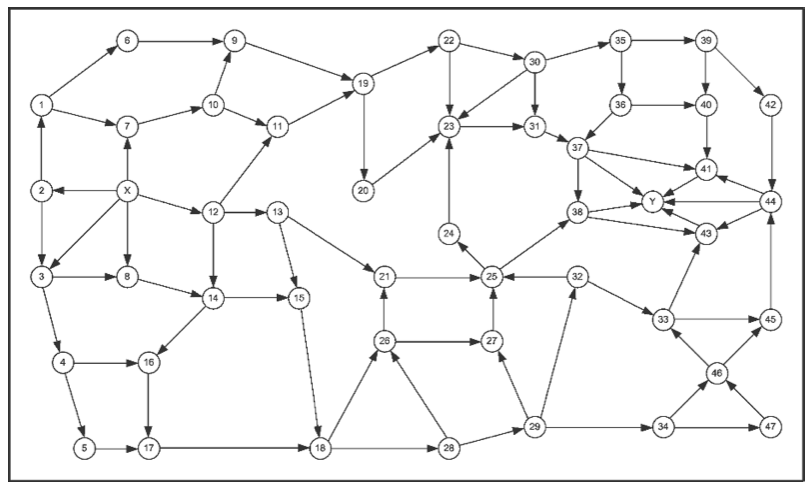
\includegraphics[scale=1]{./img/figure3-16.png}
	\caption{Road Map of the urbanized region of cities X and Y}
	\label{network3-6}
\end{figure}

\paragraph{(a)}
\begin{quote}
Determine the minimum number of checkpoints for the road system of Figure 3.16, together with their locations. What is the minimum amount of money needed for this operation.
\end{quote}

\paragraph{}
The problem is equivalent to finding the minimum number of arcs so that removing these arcs leaves X and Y disconnected. In other words, we are interested in the minimum cut between vertices X and Y. To find it we find the maximum flow in the network obtained in an obvious way from figure \ref{network3-6}. The capacities of all arcs are 1. X is the source, Y is the sink. The value of maximum flow is the minimum number of checkpoints. To find the locations of checkpoints we find all arcs from reachable to unreachable (from X) vertices in residual network. The result is shown in table \ref{mincut3-6a}. We need 4 checkpoints, so the total cost is \texteuro 1,200,000.

\begin{table}[H]
\centering
\begin{tabular}{|r|}
\hline
$18 \rightarrow 28$ \\ \hline
$19 \rightarrow 22$ \\ \hline
$23 \rightarrow 31$ \\ \hline
$25 \rightarrow 38$ \\ \hline
\end{tabular}
\caption{Optimal checkpoint locations}
\label{mincut3-6a}
\end{table}

\paragraph{(b)}
\begin{quote}
Answer the same questions as in part (a), but with the direction of traffic on the road segment 32 – 25 reversed.
\end{quote}

The optimal checkpoint locations are shown in table \ref{mincut3-6b}. The cut is trivial: no one can leave X without passing a checkpoint. The total cost is \texteuro 1,500,000.

\begin{table}[H]
\centering
\begin{tabular}{|l|}
\hline
$X \rightarrow 2$ \\ \hline
$X \rightarrow 3$ \\ \hline
$X \rightarrow 7$ \\ \hline
$X \rightarrow 8$ \\ \hline
$X \rightarrow 12$ \\ \hline
\end{tabular}
\caption{Optimal checkpoint locations}
\label{mincut3-6b}
\end{table}

\paragraph{(c)}
\begin{quote}
Answer the question in part (a), if all flow directions in Figure 3.16 are reversed, and commodity flow from Y to X is considered.
\end{quote}

\paragraph{}
It's quite obvious that nothing changes if we reverse all arcs. The result is the same as in (a).
